\subsection*{Groep server}
\begin{itemize}
\item
Admin pagina ontwerp is af (zie hieronder). Dit ontwerp wordt gebruikt als basis.
\item
De charger status is af te lezen en handmatig te veranderen vanaf de site.
\item
De sidebar met checkboxen en dropdown menu per checkbox gemaakt.
\item
In PHP gewerkt aan beveiliging tegen SQL injectie. Deze is klaar voor de SQLinsert functie.
\item
De ODROID zijde van de verbinding naar de server is klaar. Deze is getest op memory leaks. Het enige wat nog fout gaat is een foute internet connectie. Daar moet nog aan gewerkt worden.
\item
De PHP zijde van de verbinding is bijna klaar. De tabellen worden op dit moment aangepast zodat ze overeenkomen met de data vanaf de ODROID, en volgende week wordt het script afgeschreven.
\end{itemize}
Alle code van de admin pagina en de SQL functies staan op de server in de map admin\_page.
De website waarop de huidige status van de admin pagina staat heet "solarpoweredbikes.tudelft.nl/admin\_page/dashboard.php"
De code van de PHP zijde van de verbinding met de ODROID staat in de map ccon.
De c-code wordt als aparte zip meegestuurd.


\subsubsection*{Volgende week}
\begin{itemize}
\item
Data verwerken van de sidebar.
\item
Beveiligen van de andere SQL functie.
\item
Afschrijven van de PHP code en het verder aanpassen van de MySQL tabellen.
\end{itemize}

\begin{figure}[htbp]
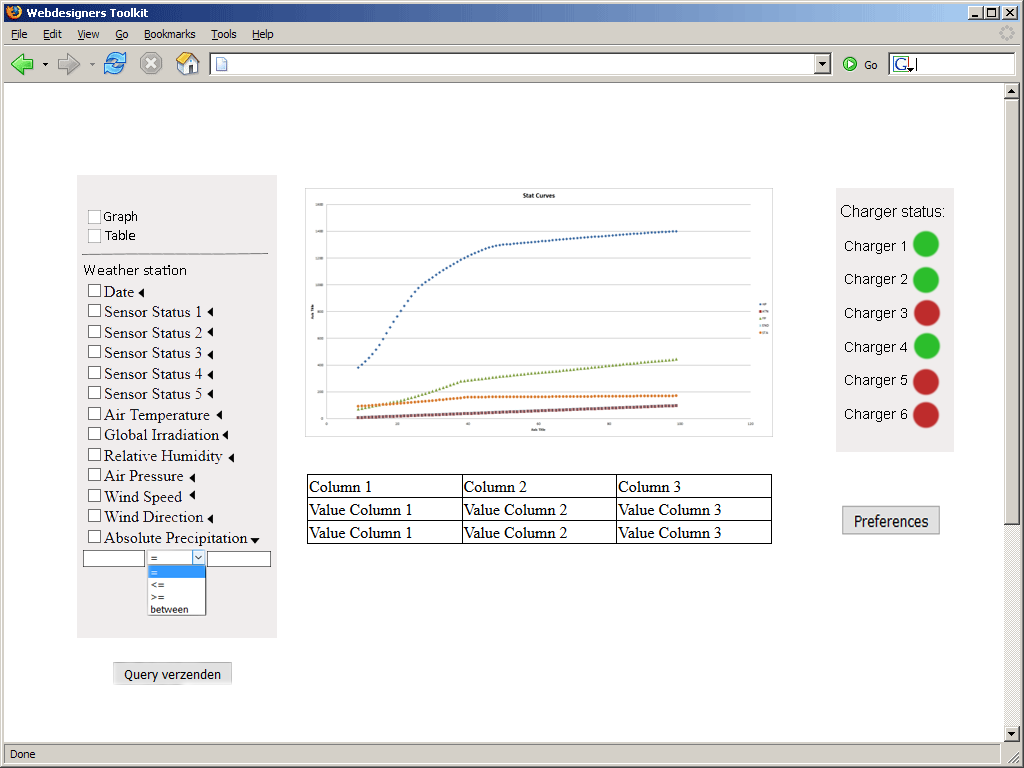
\includegraphics[width=0.8\textwidth]{adminpage}
\caption{Admin pagina ontwerp}
\end{figure}
